\newpage
\thispagestyle{empty}
\mbox{}

\ifdefined\included
\else
\setcounter{chapter}{7} %% Numéro du chapitre précédent ;)
\dominitoc
\faketableofcontents
\fi

\chapter{Interactive Social Multi-Agents Simulation for Robot Navigation: IMHuS}
\chaptermark{Intelligent Multi Human Simulation: IMHuS}
\label{chap:8}
\minitoc

\chapabstract{This chapter presents the IMHuS system designed to choreograph several agents with group movements and social behaviors. This system complements the InHuS system presented in the previous chapter by generating multi-human scenarios. This system has been qualitatively evaluated in an elevator scenario.}

\section{Introduction}

In chapter~\ref{chap:7}, we showed that the InHuS system effectively challenges robot navigation systems in intricate and human-populated environments. However, simulating the interactive agent is computationally demanding. This is why we limited the simulation to only a single intelligent agent. Nevertheless, it is also relevant to general intricate scenarios with several agents. Existing works simulating crowds are only based on a reactive approach and are not necessarily designed to be used to benchmark robot systems.

This is why we propose the Intelligent Multi-Human Simulator (IMHuS). This work is strongly inspired by and complementary to the InHuS framework presented in chapter~\ref{chap:7}. Together with two researchers from the University of Leon in Spain and an intern, we designed this framework based on InHuS. The implementation of this system has been majorly done by the intern. This system allows choreographing several interactive agents with group or individual movements and social behaviors. The individual agents are less complex and demanding than the InHuS one, allowing the simulation to run smoothly.  
This system has been evaluated in the elevator scenario, as defined for the SciRoc competition 2019.

We begin with a comparison between InHuS and this additional work while briefly describing it. After, a more formalized presentation of IMHuS is provided, detailing the information given in the prior comparison. Eventually, the elevator use case evaluation is presented. 


\section{Comparison InHuS vs. IMHuS}

\subsection{Similarities}

Let's first mention the similarities between InHuS and IMHuS work. Like InHuS, this work aims to replicate scenarios involving humans to help social robotics research. Similarly, the simulated interactive agents can be choreographed in a step-based manner to create high-level social behaviors such as waiting for an elevator, getting in and out of it, or standing in front of a store window and moving to the next one. The agents navigate in the environment while avoiding static obstacles and being reactive to moving obstacles to prevent collisions. The agents can also wait for a defined amount of time or turn to look in a direction. Like in InHuS, \textit{Attitudes} can be activated to generate specific behavior, such as harassing the robot. This work also analyzes the execution to compute metrics evaluating the robot's performance in defined social situations. The framework architecture is close to the InHuS one and can also be used with different robotic simulators. Here, it has been implemented with Gazebo.


\subsection{Differences}
However, IMHuS differs from InHuS in several ways. The primary reason is that it manages several interactive agents instead of a unique one in InHuS. Moreover, the agents can exhibit social behavior using explicit social groups. For instance, they can move together to another location or talk in pairs. This requires the new \textit{grouping} actions which create or dismantle groups of humans. An interesting addition is the implementation of asynchronous actions. They differ from synchronous actions, such as navigation/turning/grouping actions, which the agents accomplish during one specific step. Asynchronous actions are not associated with a specific step and correspond to a system of \textit{request} and \textit{response}. Thanks to them, one agent can request another to perform a specific task. For instance, the robot can request a human agent to call the elevator, or if supported, a human agent can request the robot to go somewhere. Not every agent can respond to the robot's requests. For instance, if the robot asks for someone to press the button and no one is around, the request will be dropped, counting as a failure. 

In order to handle several human agents, some simplifications were made compared to the InHuS framework. First, when navigating, IMHuS agents are reactive to other agents. However, their movements are less smooth than the InHuS agent. This is because InHuS couples a frequent global path replanning, taking into account static and moving obstacles and an elaborated local planner to follow the planned path. The local planner used is the Human-Aware robot navigation planner CoHAN, which was presented in the previous chapter. It also allows the agent to have proactive avoidance movements. Also, InHuS uses frequent global path replanning to be even more reactive and to identify sudden path blockage due to other agents. Hence, instead of blindly following the global path it can identify when its optimal path is blocked and switch into a conflicted mode where it reasons on its goal to adapt it potentially. Currently, the agent approaches the blocked spot before stopping to wait for the path to be cleared. 
On the other hand, IMHuS agents do not use any local planner and simply move at a defined speed along the updated global path. This induces human agents to sometimes move abruptly and avoid obstacles at the last moment. 
In addition, IMHuS agents' actions are dictated by the given choreography and do not have individual goal reasoning processes like in InHuS. Hence, IMHuS agents are currently incapable of identifying path blockage situations and may behave erratically in such cases.  

However, this new scheme is still very interesting because of the multitude of human agents generated and the social behaviors that can be choreographed. It can generate relevant and challenging situations for social robotics to handle.


\section{Rational}

The goal of the tool described in this paper is to provide a means to generate scenarios in which predefined social interactions of groups of reactive humans can be used to test the social performance of a robot behavior under evaluation. In the rest of the paper, we will refer to it as \textit{tested robot}. The aim is to use the system to benchmark human-robot interaction behaviors.

The goal of IMHuS, the tool described in this paper, is to provide an open-source toolkit for defining high-level reactive simulated humans with the ability to show the behavior of social groups but using realistic standard robotics simulators that allow researchers to use models of their real robots, both for debugging their algorithms and for benchmarking and repeatability.


\section{Design of a Step-based Social Simulation}
\label{sec:design}

The goal of IMHuS is to standardize the validation of autonomous robot behavior in the presence of people, allowing researchers to design repeatable human social situations. For example, we can define a set of waypoints where different simulated people arrive, meet, and move as a group to a different position, or two people facing each other and then moving together to a different location.

Our proposal considers that both individuals and groups must be included in the simulated environment and that each simulated person should exhibit adaptive behavior in both cases. To achieve this goal, we assume that global path planning for the whole set of agents is more suitable for defining fixed social behaviors than the individual path planning approach. This assumption also serves the purpose of humans exhibiting a typical social behavior that the robot must be able to detect in order not to cross, for example, through the middle of a social group.

A central process can have perfect knowledge of the simulated environment, accessing the real and accurate positions of all the elements of the simulations (obstacles, robots, etc.). It is not designed to emulate an embedded agent since the robot simulation process has to obtain the information through the noise-simulated sensor readings provided by the simulator. This process can use the API of the simulator to get all the information directly, without noise and identification problems (it will know which types of elements are in the simulation and their state). For instance, it does not need to identify if something is ``a door" or if it is opened. The door state is obtained directly from the simulator.


\subsection{Choreography Oriented Simulation}

The constraints and assumptions made for IMHuS are:
\begin{enumerate}
    \item The set of persons $P=\{p_1, p_2, ... p_n\}$ in the environment is defined {\em a priori}, and each person will be unequivocally identified by its ID ($p_i$) during each execution.
    \item The number of locations $L=\{l_1, l_2...,l_m\}$ for these people is also known {\em a priori}.
    \item The number of locations will be greater than the number of people $|L| \geq |P|$.
    \item In a given time-step, only one person can stay at an individual location $l_i$.
    \item Group locations $L^n_i$ will have a maximum number $n$ of individual positions $l_1, l_2, ..., l_n$. For instance, an elevator with four positions will be named $L^4$.
    \item The number of actions is also finite and known.
\end{enumerate}

The tool aims to give researchers a high-level definition of a ``choreography'' of people moving in a social way. For instance, let's consider an example: first, a set of people ($p_1$ to $p_4$) is defined. In the first step, $p_1, p_2$ and $p_3$ must move from their initial positions to a ``group location'' ($L^3$). This joint navigation is represented in figure \ref{fig:diagram} as a continuous top-opening box grouping the three people at time-step $t_0$ and a double arrow labeled with the goal destination. In the same way, $p_4$ will remain in its position but will face a particular direction (30 degrees), indicated by the circle with an arrow. 

 \begin{figure}[h!]%
    \centering
    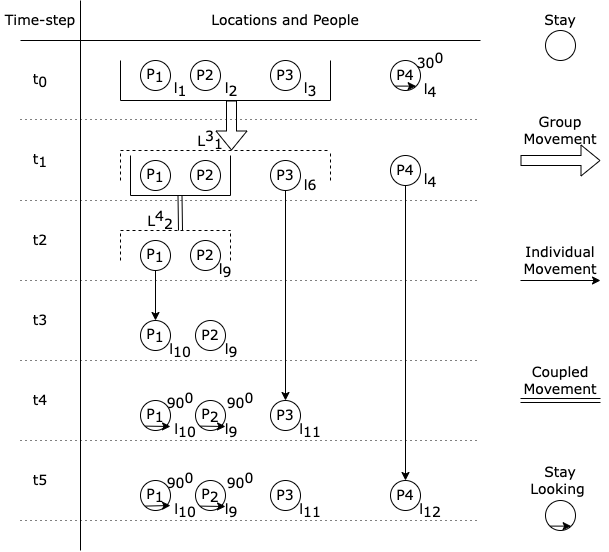
\includegraphics[width=0.7\textwidth]{Chapter8/diagrama.png}
    \caption{Schematic representation of the definition of a social navigation choreography}
    \label{fig:diagram}
\end{figure}

At $t_1$, $p_1$ and $p_2$ engage in a pair-move to $L^4$, while $p_3$ and $p_4$ initiate individual moves, indicated by a single arrow. A pair-move is a specific type of group move included in the design because it is usually the most common and can be considered the smallest group unit. At $t_2$, the two persons moving as a pair would have reached their destination, and $p_1$ will initiate its movement towards $l_{10}$, while $p_2$ remains in its current position with no particular orientation (indicated by a circle with no arrow), and $p_3$ and $p_4$ continue to navigate to their targets.

$p_1$ at $t_2$ begins to move individually towards $l_{10}$, which reaches at $t_3$ while $p_3$ and $p_4$ continue to execute their solo movement. $p_3$ reaches $l_{11}$ at $t_4$, when $p_1$ and $p_2$ begin to face in the same direction. Finally, at $t_5, p_4$ reaches its destination ($l_{12}$) and the choreography ends.

Time-step ($t_i$) in figure \ref{fig:diagram} means ``\emph{choreography steps}'', that is, significant moments for the definition of the simulation. It does not refer to a magnitude measured by a clock. We will refer to them as \emph{steps}, which is an increased ordered sequence of discrete points in time at which a given set of events has to occur. For example, $step_0$ usually specifies the initial state of all the elements of the simulation, i.e., the position of the robot, human', and the other elements. A typical step specifies a set of actions that are initiated at that instant, a navigation task for one of the humans, for instance, at $step_1$ ($t_1$ in figure~\ref{fig:diagram}).


This is the type of simulation that the tool should be able to generate. Figure~\ref{fig:imhus_architecture} shows the general architectural framework. This tool receives the definitions of the social scenarios in a definition file (an XML in its current version). It then manages the simulation, obtains the simulation data, uses existing libraries and other tools (such as $move\_base$ to calculate trajectories in \acrshort{ros}), and finally generates the log data for evaluation.

\begin{figure}[h!]%
    \centering
    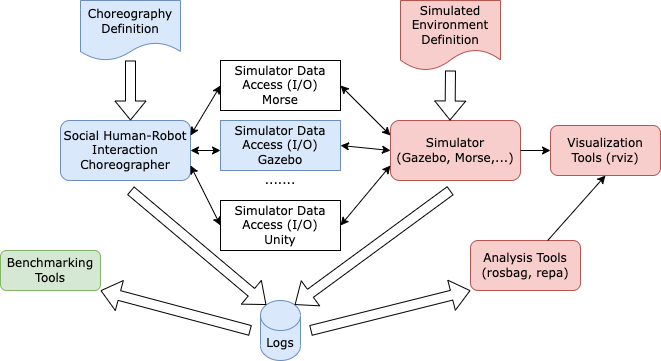
\includegraphics[width=\textwidth]{Chapter8/architecture.png}
    \caption{Global simulation architecture. Red signifies existing tools. Blue components are those described in this paper. Green signifies ongoing development. Uncolored boxes are alternative simulators under consideration.}
    \label{fig:imhus_architecture}
\end{figure}

The definition of the choreography shown in the upper left of the figure \ref{fig:imhus_architecture} is defined in XML. The design allows five types of \emph{basic actions} that the \emph{agents} (simulated robots or simulated people) can perform:

\begin{description}
    \item[Navigation actions]: Those actions modify the global pose of the agents in the environment. Typical actions in this group are $GoToPose$ and $Wait$.
    \item[Turning actions]: Actions related to the facing of the agents, such as $LookAt$ and $Turn$, depending on the way the action is specified.
    \item[Grouping actions]: These actions manage the creation and dismantling of groups.
    \item[Attitude actions]: Actions modeling the high-level behavior of the agent. For instance, a simulated human can be ordered to \textit{harass} the robot.
    \item[Synchronous actions]: Actions related to the environment to be accomplished by an agent during one specific step of the simulation. They have been standardized as $publish$ and $subscribe$.
    \item[Asynchronous actions]: Actions related to the environment and not associated with a specific step in the timeline of the simulation. They have been standardized as $request$ and $respond$.
\end{description}

These actions can be applied to a single agent or a group. Basic actions can be integrated into a $compound\_task$. For defining these actions, the following components are used:
\begin{itemize}
    \item \emph{map}: corresponds to the ``world" where the simulation will happen. Inside the map, a set of \emph{objects} can be defined, specifying their individual ID.
    \item \emph{poses}: correspond to the ``location" used in figure \ref{fig:diagram}. They comprise the $x,y$ position and orientation $\theta$ and a $radius$ of tolerance for the motion planner to consider that the goal has been reached.
    \item \emph{agents}: that can be either $robots$ or $humans$, each of them identified by an unique ID. They are given an initial pose where they appear in the world.
    \item \emph{groups}: they can be created and dismantled during the simulation
\end{itemize}

The evolution of the simulation is based on steps, as described in the previous section. The regular steps are synchronous, but there is an asynchronous step for interacting with the tested robot:
\begin{itemize}
    \item A scenario is composed of a set of regular steps and a singular asynchronous step.  
    \item Steps are made up of different actions like navigation, grouping, etc.
    \item Every action of a step is executed {\em at the same time}, meaning that the actions are executed in simulated parallelism. 
    \item One step ends when all its actions have finished.
    \item The asynchronous step runs in parallel to the execution of the synchronous steps. 
    \item The scenario ends when the last regular step ends.
\end{itemize}

\section{Implementation}
\label{sec:implementation}
In the current version, choreographies are defined in an XML file that includes four main sections:
\begin{itemize}
    \item Map = poses and objects. Example: poses definition.
    {\footnotesize
        \begin{quote}
        \begin{verbatim}
<poses> ::= <pose> (<pose>)* ;
    <pose> ::= <poseID> <x> <y> <theta> <radius> ;
        \end{verbatim}
        \end{quote}
    }
    \item Agents = humans/choreographed robots with their initial poses and groups with their composition. Example: group definition.
    {\footnotesize
        \begin{quote}
        \begin{verbatim}
<groups> ::= (<group>)* ; 
    <group> ::= <groupID> <pair> (<human> (<human>)*) ;
        <pair> ::= <pairID> <human> <human> ;
        \end{verbatim}
        \end{quote}
    }
    \item Tasks = generic actions. Example: compound tasks and look-at action definition.
    {\footnotesize \noindent
        \begin{quote}
        \begin{verbatim}
<compound_tasks> ::= <compound_task>* ;
    <compound_task> ::= <compound_taskID> <action> (<action>)*;
<lookAt_action> ::= <actionID> (<humanID>|<robotID>|<objectID>); 
        \end{verbatim}
        \end{quote}
    }
    \item Scenarios = step elements of synchronous steps and asynchronous steps. Example: scenario definition. 
    {\footnotesize
        \begin{quote}
        \begin{verbatim}
<scenario> ::= <name> <step> (<step>)* (async_step);
    <step> ::= <stepID> <stepElement>; 
        <stepElement> ::= <agentsID> <pose>|<compound_task>;
        <agentsID> ::= <humanID>|<robotID>|<pairID>|<groupID>;
    <async_step> ::= <respond_event_action>;
        \end{verbatim}
        \end{quote}
    }
\end{itemize}

The prototype has been implemented as a new version of the InHuS tool (\cite{favier_SSC}), which connects to the Gazebo simulator to obtain information about the world. It uses the \emph{move\_base} \acrshort{ros} to generate the global plan for each agent and updates the positions of each agent in the next step of the simulation accordingly. The new version is capable of handling the navigation of multiple agents (humans) in parallel while managing conflicts and completing individual tasks as in the previous version. It also provides an updated graphical user interface for repeatedly selecting and executing scenarios defined in the XML file.

The IMHuS tool shown in Figure~\ref{fig:imhus} has been structured in three layers: the IMHuS layer (in blue), its configuration in the application layer (in yellow), its communication with the simulator and \acrshort{ros} (in red). The robot whose behavior would be tested in the tool has also been included (in violet).

  \begin{figure}[ht]%
     \centering
     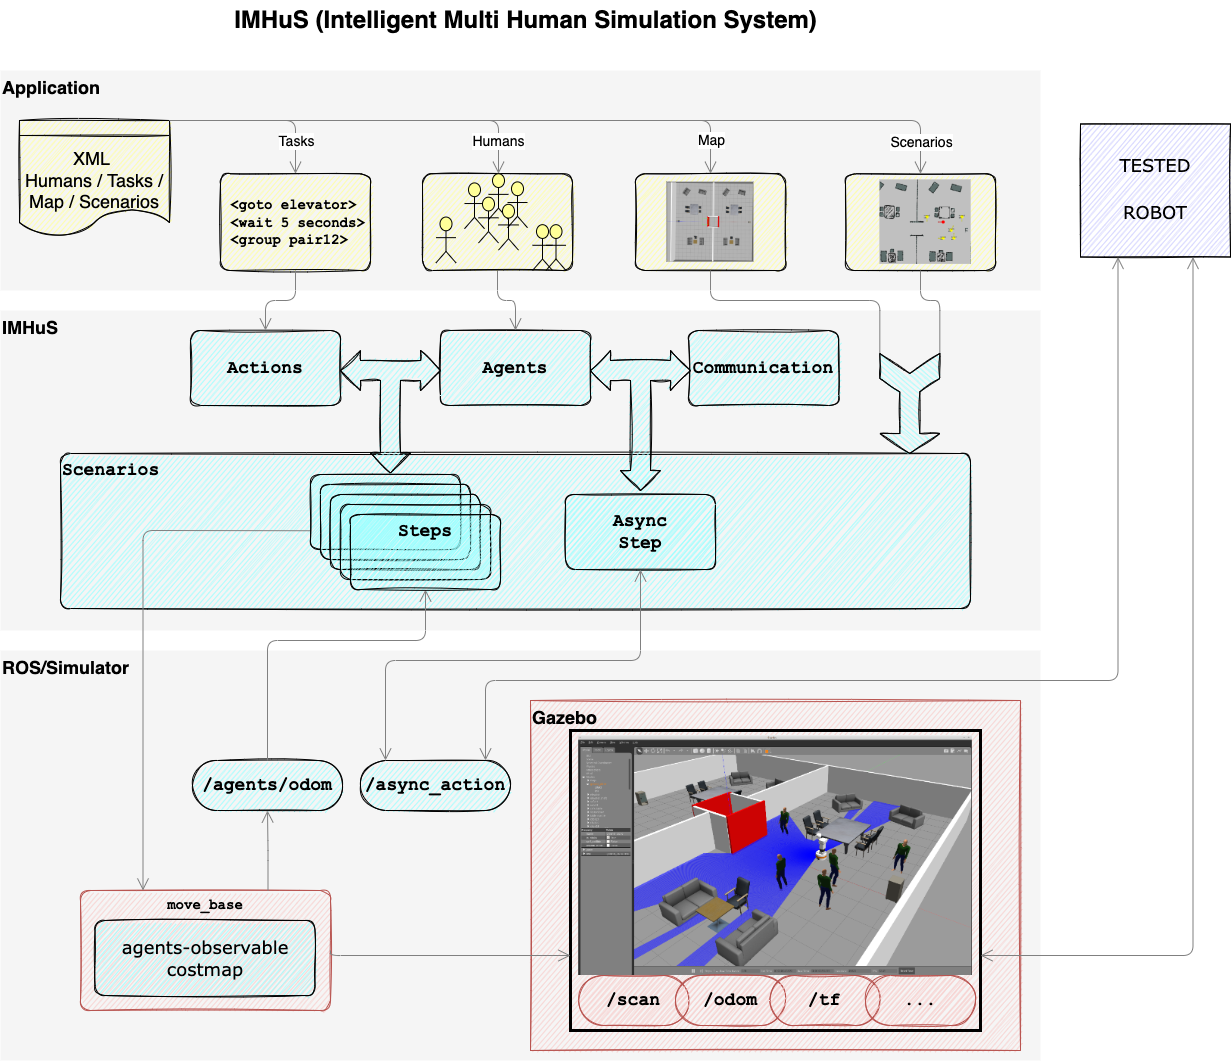
\includegraphics[width=1\textwidth]{Chapter8/IMHuS.png}
     \caption{Structure of the new IMHuS tool.}
     \label{fig:imhus}
 \end{figure}

\begin{description}
    \item[Application layer] This layer includes the XML configuration file needed to use IMHuS by defining its main components: map, agents, tasks, and scenarios. The map includes all the locations of the agents to be used during the choreography and those of static objects. These locations are represented as poses, and a name is assigned to each. The description of the agents includes the name, and initial position of all humans and robots choreographed, as well as the name and composition of the groups that will appear at any step. Generic tasks are described with no specific subject to perform them so that several agents can reuse them. Lastly, the scenarios describe the choreography steps. Each step includes a set of tasks assigned to a particular agent or a group. They are the step elements. 
    \item[IMHuS layer] The tool interprets the information contained in the XML configuration file to represent the tasks as actions and the humans/robots as agents. When the scenarios are run, a command combines actions with agents for every step element. The commands concerning each agent are executed in a separate thread inside a step. The step finishes when all the threads are done. This is the way simultaneous movements of agents are achieved. 
    This is the behavior of the tool for the choreography, but considering that the tested robot will be present, there must be a way for it to communicate with the simulation agents, just as it would happen in the real world. The asynchronous step is responsible for this task. At any point, the tested robot can ask something, for example, to press the elevator button. This action would be done through the communication module and answered by the agents in the simulation in this asynchronous step by a response action. Not every agent can respond to a request from the tested robot. For instance, if the robot asks for someone to press the button and no one is around, the request will be dropped, counting as a failure.
    \item[ROS/Simulator layer] IMHuS uses this layer to place the agents in the simulation, ask for the trajectories to move them around, and communicate with the tested robot. The agents are placed in the world as obstacles so that they are avoided when \texttt{move\_base} is asked for a new path. The costmap obstacle layer has been modified to obtain what we call the \textit{agents-observable costmap} that IMHuS needs.
    \item[Interface of the tested robot] The way to include the software of a robot in the simulator for its social behavior to be tested would be through the simulator, here Gazebo. Outside the simulator, the only communication would be through asynchronous actions. They allow the robot to send a request action to be answered by a response action from one agent of the simulation.
\end{description}


\section{Use Cases}
\label{sec:useCases}


This module is available as Open Source, and it has been evaluated in the elevator scenario, as defined for SciRoc competition (\href{https://github.com/LAAS-HRI/IMHuS}{IMHuS repository link}). %In this scenario, the robot has to be able to take an elevator in the presence of people.

An elevator scenario will be used to show a running example of the behavior of the IMHuS system with a tested robot and also to explain the communication between the \textit{tested robot} and the agents of IMHuS (video available at \href{https://github.com/LAAS-HRI/IMHuS/videos}{this link}). The proposed scenario includes five human agents and the \textit{tested robot}, whose goal is to go to the second floor. In order to do that, it has to ask a human agent to push the elevator button. Figure~\ref{fig:take_elevator_video_1} shows the initial situation where the \textit{tested robot} is approaching the elevator, human\_2 is walking, and the rest of the humans are idle.

\begin{figure}[!ht]
  \centering
  {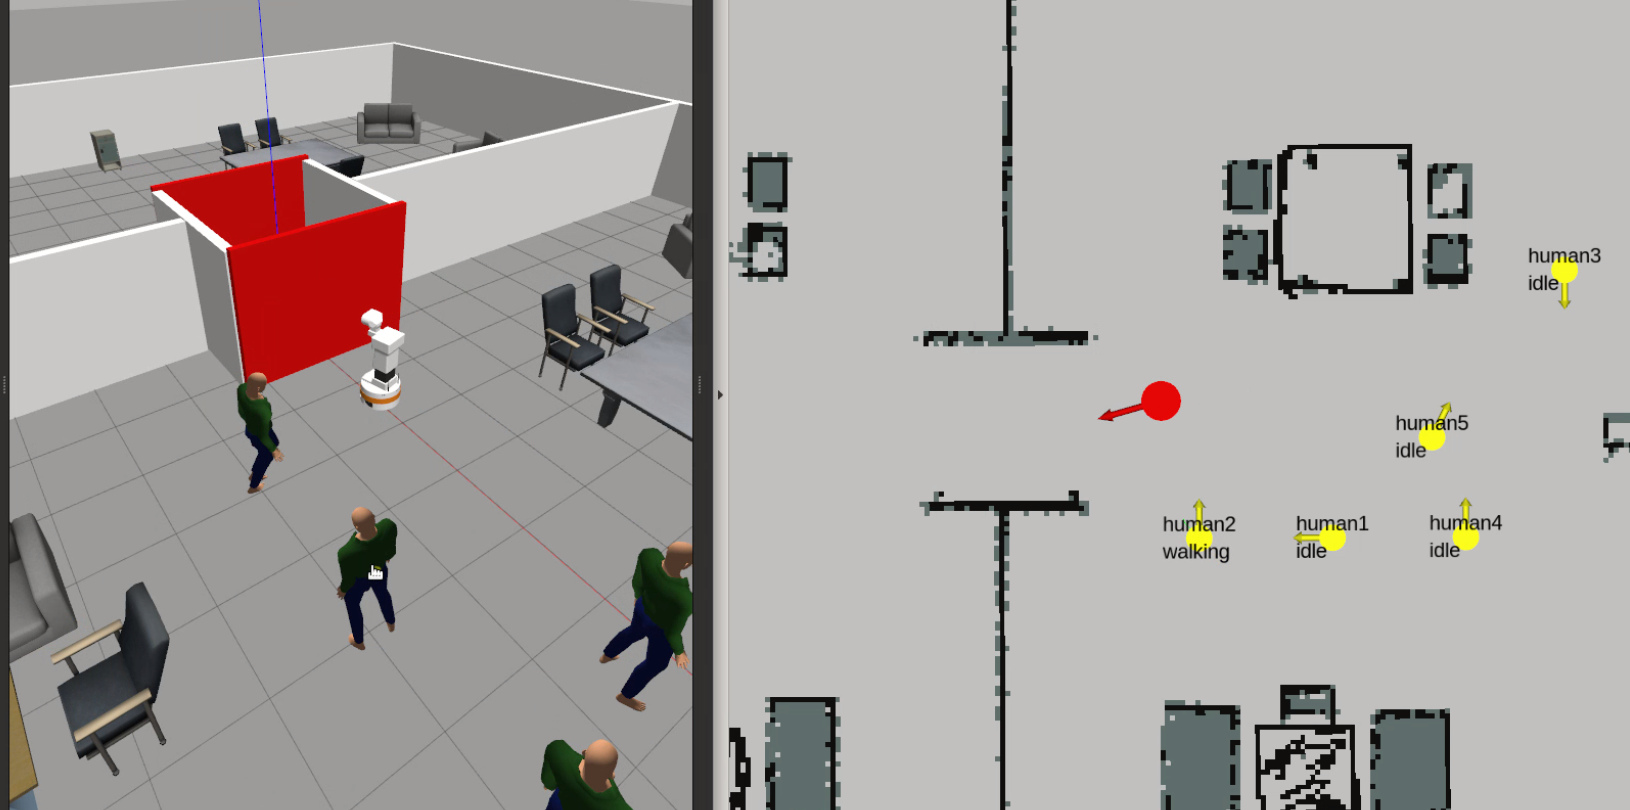
\includegraphics[width=1\textwidth]{Chapter8/seq1.png}}\\
  \caption{Initial situation.}
  \label{fig:take_elevator_video_1}
\end{figure}

Once the \textit{tested robot} gets to the elevator door, it requests that one of the humans perform an action. In order for a \textit{tested robot} to trigger an action in IMHuS, it has to publish a specific message type on the \texttt{async\_action} topic (see Figure~\ref{fig:imhus}). Doing so triggers an asynchronous action response from IMHuS. This message should contain the time of emission, the name of the agent requesting it, the pose of this agent, and the name of the task it is requesting. If the scenario includes in its configuration an asynchronous action response corresponding to the requested action, that action is triggered on the human's side.

At this point, two different things can happen. If there is no human close enough to the \textit{tested robot}, or there is a human but it is not in an idle state, no one will respond to the request, and it will be dropped, as Figure~\ref{fig:take_elevator_video_2} shows.

\begin{figure}[!ht]
  \centering
  {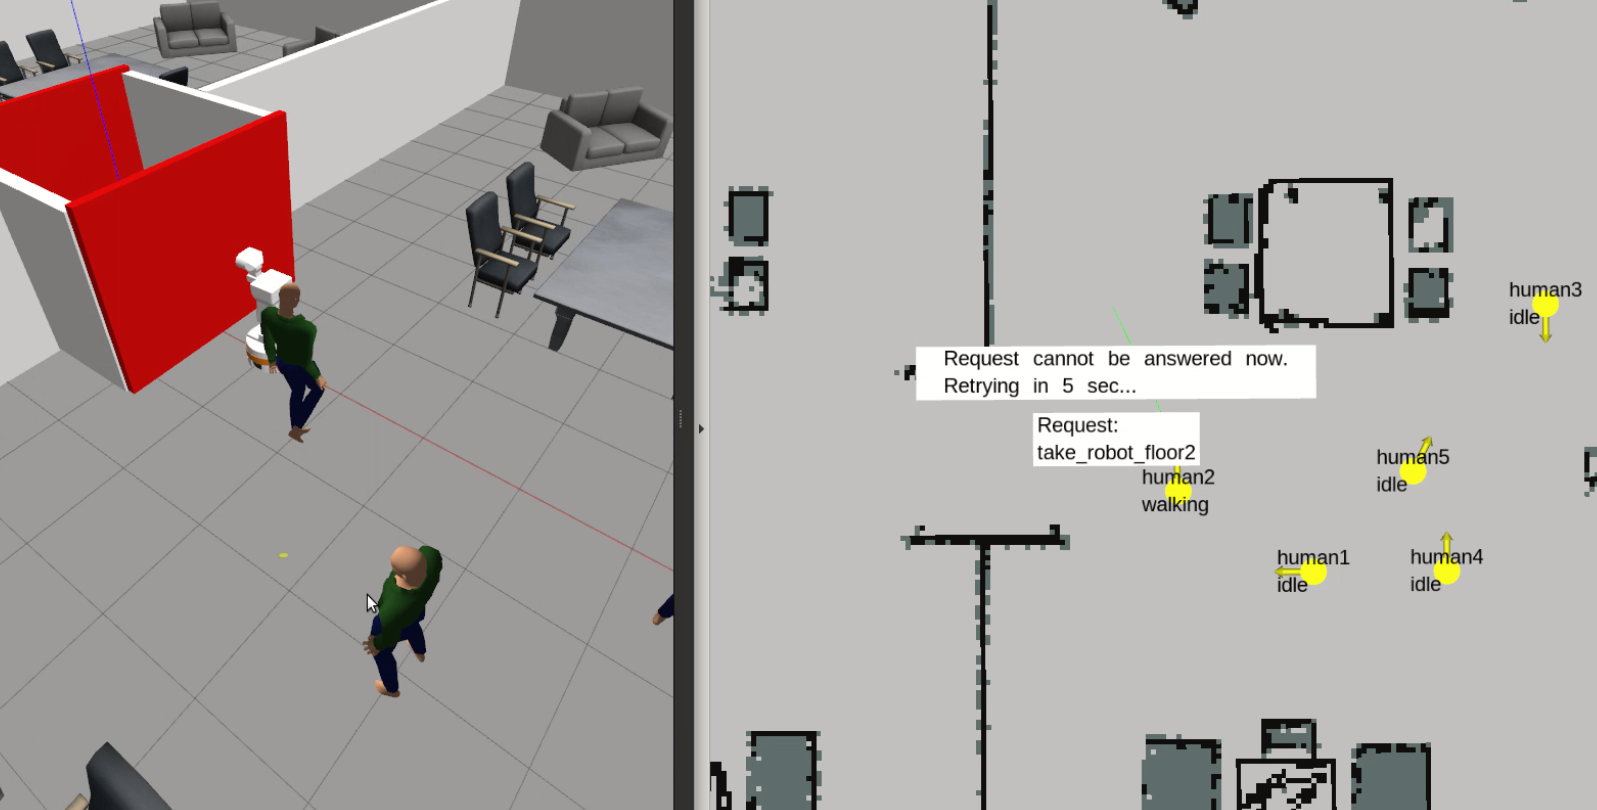
\includegraphics[width=1\textwidth]{Chapter8/seq2.png}}
  \caption{Request dropped.}
  \label{fig:take_elevator_video_2}
\end{figure}

The \textit{tested robot} repeats the request every five seconds until human\_2 enters an idle state and responds to the request. Figure~\ref{fig:take_elevator_video_3} shows this moment of the simulation. When an asynchronous action request is triggered, IMHuS periodically checks if one human is able to respond. The requirements for a human agent to respond are to be in the idle state and within a $3m$ radius from the \textit{tested robot} position when it requested the action. If several human agents can accept the task, the task will be assigned to the closest human.

\begin{figure}[!ht]
  \centering
  {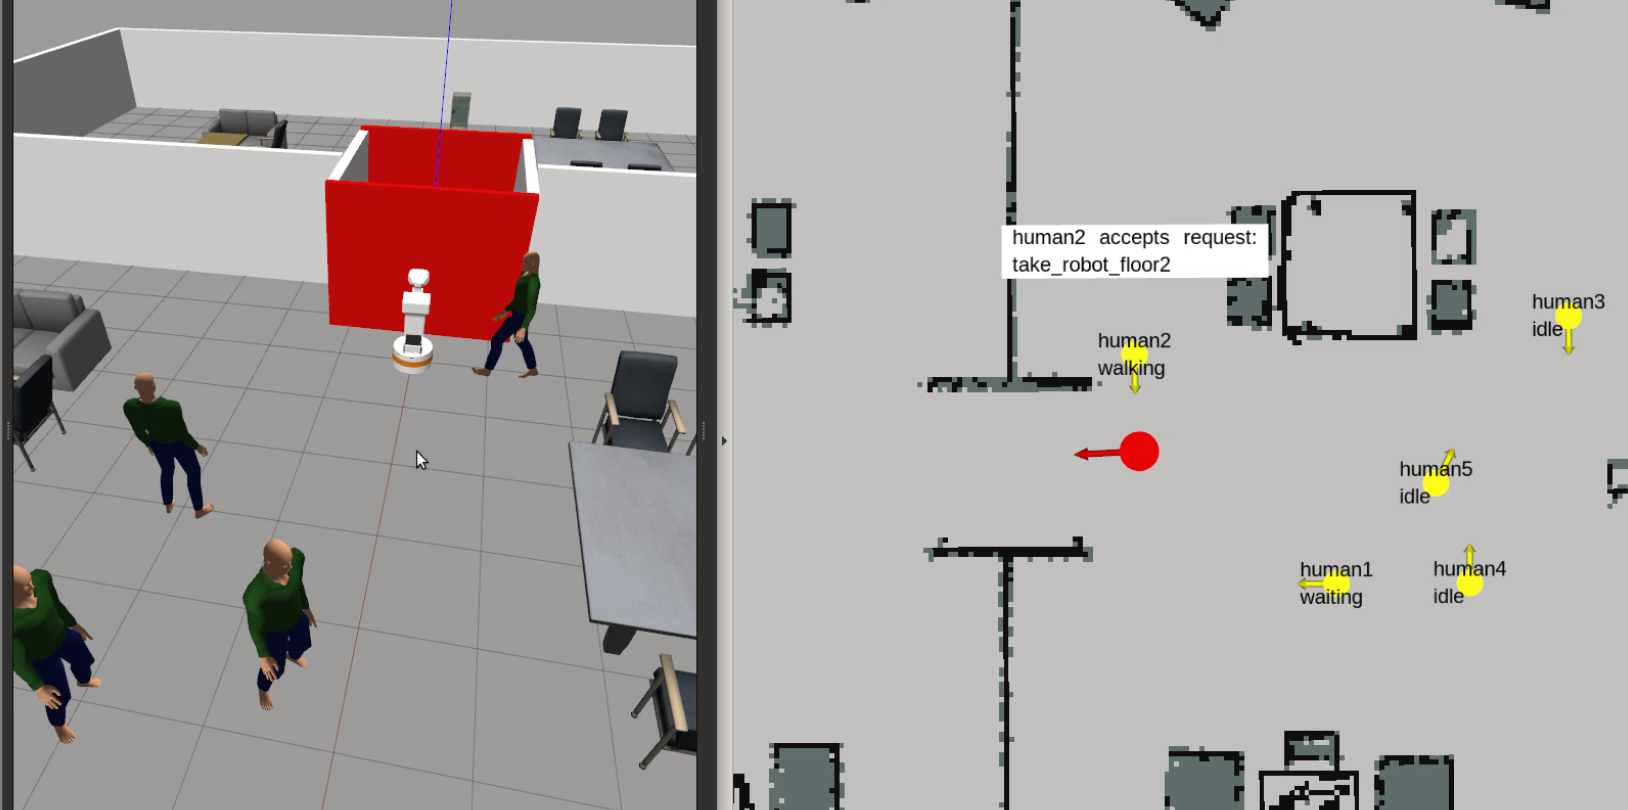
\includegraphics[width=1\textwidth]{Chapter8/seq3.png}}\\
  \caption{Request accepted by human2.}
  \label{fig:take_elevator_video_3}
\end{figure}

Figure~\ref{fig:take_elevator_video_4} shows the final situation where the \textit{tested robot} has reached the second floor, simulated in the scenario as the room on the other side of the elevator.

\begin{figure}[!ht]
  \centering
  {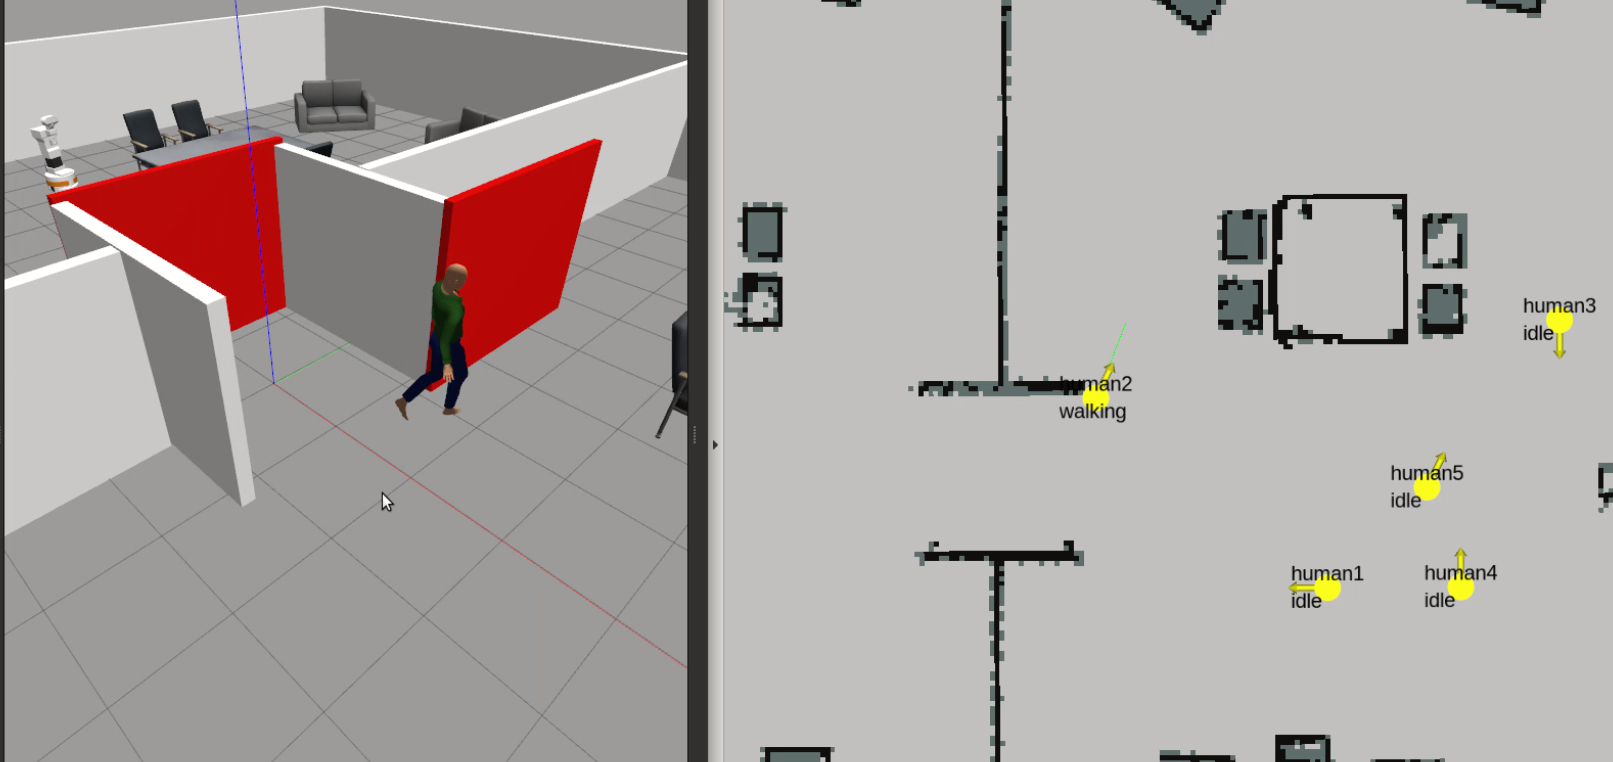
\includegraphics[width=1\textwidth]{Chapter8/seq4.png}}\\
  \caption{Final situation. \textit{Tested robot} in second floor.}
  \label{fig:take_elevator_video_4}
\end{figure}

\section{Conclusions and Future Work}
\label{sec:conclusions}

The proposed tool, IMHuS, offers the possibility to create a realistic and challenging simulated environment in which groups of humans can be choreographed to evaluate the behavior of a \textit{tested robot}. Different scenarios can be easily created using an XML configuration file in which social situations can be defined to measure the behavior of \textit{tested robots} in a replicable environment. Furthermore, human agents are programmed to respond to interactions related to the particular situation of each scenario and their communication with the \textit{tested robot}. 

IMHuS's code is available as Open Source in the  \href{https://github.com/LAAS-HRI/IMHuS}{IMHuS repository}. The current version has been implemented for the Gazebo simulator, but the design presented in section~\ref{sec:design} can be easily migrated to other simulators, such as MORSE or Unity. The tool could be used to benchmark competitions such as SciRock or RoboCup as a previous step for the teams before getting to the physical robot challenges. To create a new scenario with IMHuS, all that is needed is a map and the configuration file to choreograph the human agents. The software has been designed to easily support the addition of both new tasks to be performed by the humans and new interactions between them and the \textit{tested robot}.

One of the ongoing developments is the automatic generation of simulation metrics such as the distance between the robot and the agents, time-to-collision, etc. Another line of work is the extension of basic actions, especially towards the social behavior of groups of agents. Last, IMHuS is being tested with CoHAN \cite{singamaneni2021human}, a human-aware robot navigation planner, to challenge CoHAN under several human-robot interaction settings. From this, we plan to identify the areas of improvement for human-aware navigation planners and provide a benchmark for testing these planners.
